\documentclass{article}

\usepackage{a4wide}
\usepackage[utf8]{inputenc}
\usepackage[T1]{fontenc}
\usepackage[french]{babel}
\usepackage[babel=true]{csquotes} % guillemets français
\usepackage[export]{adjustbox}% http://ctan.org/pkg/adjustbox
\usepackage{graphicx}
\graphicspath{{image/}}
\usepackage{color}
\usepackage{hyperref}
\usepackage[section]{placeins}
\hypersetup{colorlinks,linkcolor=,urlcolor=blue}

\usepackage{amsmath}
\usepackage{amssymb}

\title{Rapport de Développement mobile}
\author{Fr\'ed\'erick Fabre Ferber , L3 Informatique}

\begin{document}

\maketitle

\begin{abstract}

Le but de ce rapport est de présenter l'élaboration d'une application mobile sur deux systèmes différents. 
L'un sous \textbf{Android} en \textbf{Java} et l'autre sous \textbf{iOS} en \textbf{Swift}.

\vspace{1\baselineskip}

L’application décrite ici est un \textbf{Mastermind} où l'on devra deviner une combinaison de 4 couleurs aléatoires pour ensuite pouvoir inscrire son nom et le temps que l'on aura mis pour deviner la combinaison dans une liste de scores. 

\vspace{1\baselineskip}

\textit{Durant ce rapport nous verrons les détails de l'application pour les deux \textbf{plateformes}.}

\end{abstract}

\section{Fonctionnement général de l'application}

\subsection{Principe et règles du Mastermind}
\label{subsection : Principe et règles du Mastermind}

\textbf{Mastermind} est un jeu de société à deux joueurs créé 1972. Le premier joueur va élaborer une combinaison de 4 couleurs parmi les différents pions de couleurs disponible. Le deuxième joueur doit alors trouver cette combinaison c'est-à-dire les bonnes \textbf{couleurs} aux bonnes \textbf{positions}. 

\vspace{1\baselineskip}

Pour cela, il va introduire 4 pions sur une rangée, viens ensuite \textit{l'arbitrage} du second joueur, en effet celui-ci va déterminer si les pions de la rangée sont conformes à la combinaison en plaçant des pions dans la grille d'arbitrage : 

\vspace{1\baselineskip}

\begin{itemize}

\item Un pion \textbf{Blanc} si la couleur du pion n'est pas dans la combinaison.
\item Un pion \textbf{Rouge} si la couleur du pion est dans la combinaison mais est mal placée.
\item Un pion \textbf{Noir} si le pion est bien placé et à la bonne couleur. 

\end{itemize} 
\vspace{1\baselineskip}

\textit{\textbf{Attention :} la couleur des pions pour l'arbitrage diffère beaucoup d'une version de Mastermind à une autre, durant tout le rapport et dans l'application nous utiliserons cette manière d'arbitrer. }

(Voir \ref{fig:Grille d'un mastermind avec les rangées de pions de couleurs au centre et les pions d'arbitrage à droite})

\vspace{1\baselineskip}

Le joueur doit alors trouver la bonne combinaison en s'aidant des pions mis sur la grille d'arbitrage. S'il ne trouve pas en 10 manches, il a alors perdu. 

\begin{figure}[tb!]

\centering{ 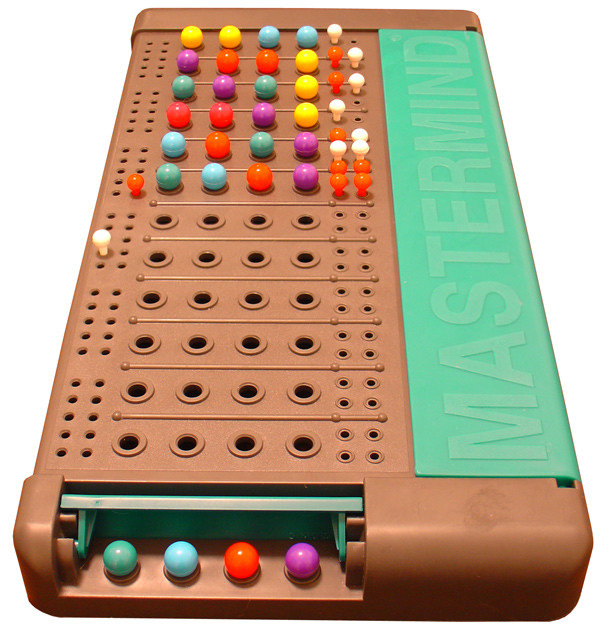
\includegraphics[scale=0.2]{img/Mastermind.jpg}}

\caption {Grille d'un mastermind avec les rangées de pions de couleurs au centre et les pions d'arbitrage à droite \label{fig:Grille d'un mastermind avec les rangées de pions de couleurs au centre et les pions d'arbitrage à droite}}

\end{figure}

\subsection{Description de l'application} 
\label{subsection:Description de l'application}

Nous avons présenté le principe général du Mastermind dans le but d'expliquer le fonctionnement de notre application. 

Elle aura 5 écrans (une \textit{Vue} sous iOS et une \textit{Activité} sous Android) énumérés ci-dessous : 
\vspace{1\baselineskip}

\begin{itemize}

\item \textbf{Le menu d’accueil} : C'est un menu constitué de trois boutons, un bouton \textit{Jouer} qui amène à l'écran principal qui est le jeu Mastermind, un bouton \textbf{Règle} qui présente simplement les règles du jeu et un bouton \textbf{Scores} qui présente les différents scores de joueurs. (Voir figure \ref{fig:Menu})

\begin{figure}[tb]
    \centering
    \begin{tabular}{cc}
      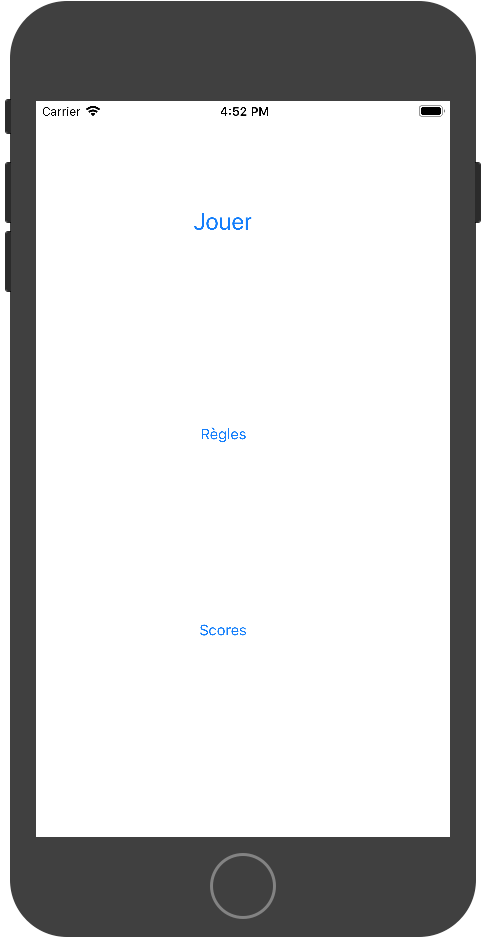
\includegraphics[width=.3\linewidth]{./img/mastermind_menu_ios.png} &
      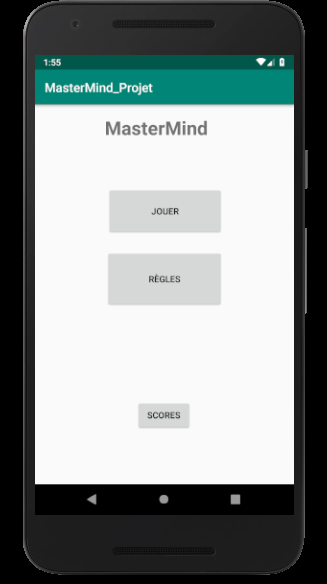
\includegraphics[width=.3\linewidth]{./img/mastermind_menu_android.png} \\
      (Menu iOS) & (Menu Android)\\
    \end{tabular}
    \caption{Menu du jeu en iOS et Android \label{fig:Menu}}
\end{figure}
\vspace{1\baselineskip}

\item \textbf{Le jeu Mastermind} : Comme dit précédemment, c'est l'écran où le jeu se déroule le jeu. Contrairement au jeu classique, on ne joue qu'a un seul joueur et le but est de déterminer la combinaison qui est générée aléatoirement. 
\vspace{1\baselineskip}
On y retrouve une grille de 10 rangées de 4 boutons qui sont notre grille de jeu, la même grille mais avec des boutons plus petits qui sont notre grille d'arbitrage. En bas de l'écran, nous avons 4 boutons de couleurs, lorsque l'on appui dessus la couleur des boutons change et on peut ensuite valider notre manche en cliquant sur le bouton \textbf{Valider} (\textit{Ce sont les seuls boutons dans cet écran qui ont une interaction avec le joueur}). Chaque fois que l'on appuiera sur le bouton \textbf{Valider} la rangée correspondante à la manche prendra la couleur des 4 boutons et l'arbitrage se mettra en place. (Voir \ref{subsection : Principe et règles du Mastermind} pour l'arbitrage).Pour finir un Timer est situé en haut à droite de l'écran qui nous servira de score. 
\vspace{1\baselineskip}
Si le joueur arrive a deviner la combinaison il gagne et passe à l'écran suivant sinon il revient au menu principal. (Voir figure \ref{fig:Jeu})
\vspace{1\baselineskip}

\begin{figure}[tb!]
    \centering
    \begin{tabular}{cc}
      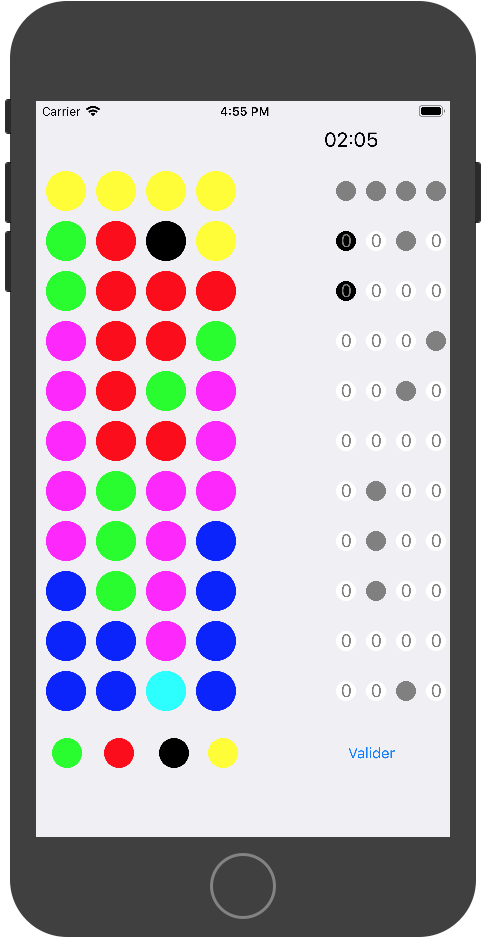
\includegraphics[width=.3\linewidth]{./img/mastermind_jeu_ios.png} &
      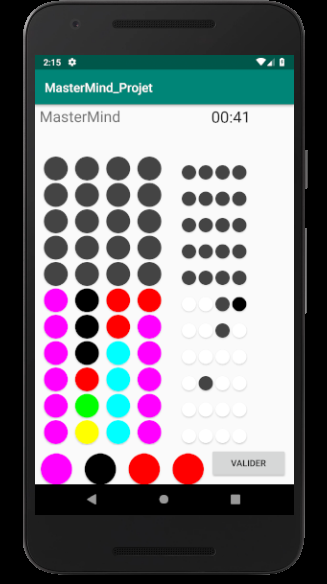
\includegraphics[width=.3\linewidth]{./img/mastermind_jeu_android.png} \\
      (iOS) & (Android)\\
    \end{tabular}
    \caption{Jeu Mastermind en iOS et Android \label{fig:Jeu}}
\end{figure}

\item L'écran \textbf{Gagner} : Lorsque que l'on a deviné la combinaison, on gagne le jeu ce qui nous amène à cet écran. Il est composé d'un texte disant que l'on a gagné avec le temps écoulé pour y parvenir. Nous devons mettre notre nom dans un champ prévu à cet effet, on appuiera alors sur un bouton pour rajouter notre nom et le temps à notre liste des scores. (Voir figure \ref{fig:gagne})

\begin{figure}[tb!]
    \centering
    \begin{tabular}{cc}
      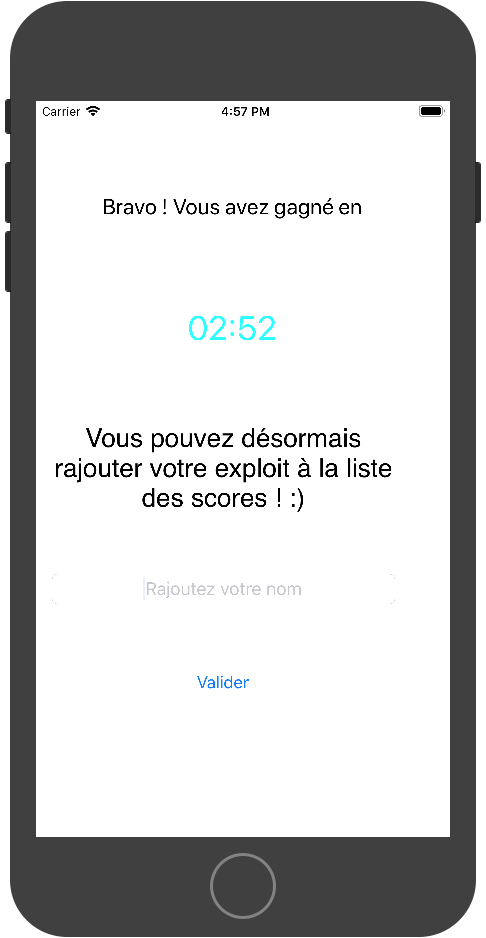
\includegraphics[width=.3\linewidth]{./img/mastermind_score_ios.png} &
      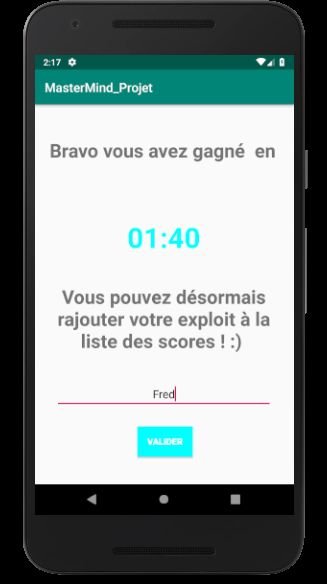
\includegraphics[width=.3\linewidth]{./img/mastermind_score_android.png} \\
      (iOS) & (Android)\\
    \end{tabular}
    \caption{Ecran \textbf{gagner} avec le nom à rentrer dans un champ. \label{fig:gagne}}
\end{figure}

\item La liste des scores : La liste des scores référence tous les joueurs ayant gagné à notre application Mastermind en marquant le \textit{nom} du joueur et le \textbf{temps} qu'il a mis pour finir le jeu dans une liste. On a un bouton \textbf{Quitter} pour revenir au menu principal. (Voir figure \ref{fig:liste})

\begin{figure}[tb!]
    \centering
    \begin{tabular}{cc}
      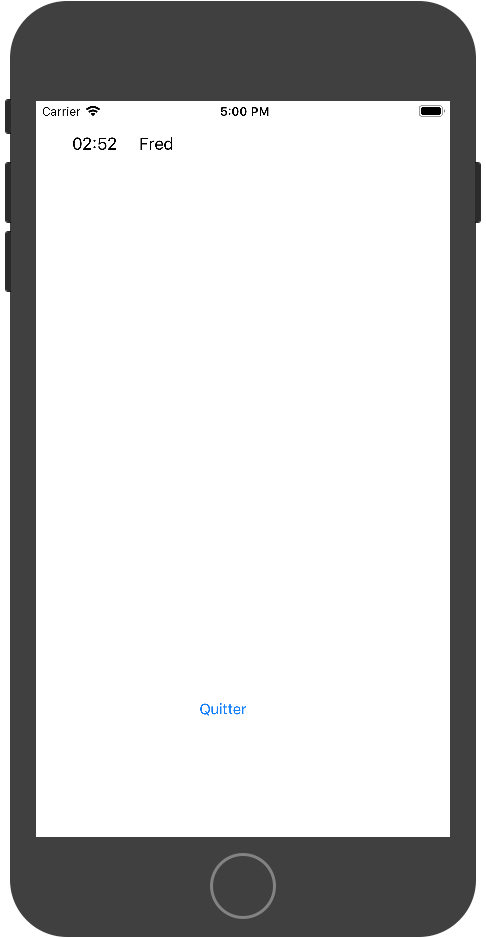
\includegraphics[width=.3\linewidth]{./img/mastermind_liste_ios.png} &
      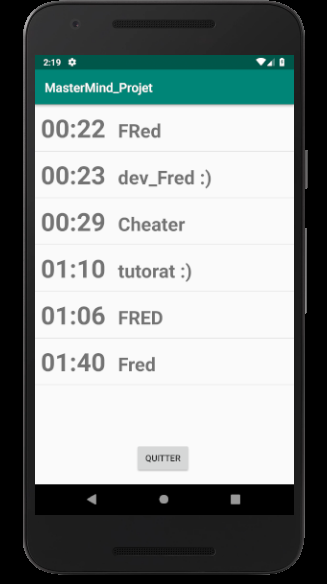
\includegraphics[width=.3\linewidth]{./img/mastermind_liste_android.png} \\
      (iOS) & (Android)\\
    \end{tabular}
    \caption{Liste des scores avec des scores rentrés par d'autres joueurs \label{fig:liste}}
\end{figure}

\end{itemize}

\section{Architecture de l'application}

Nous avons vu le principe général de l'application nous allons pouvoir voir maintenant les détails de son architecture. Nous allons décrire chacune des \textbf{Vues}/\textbf{Activités}. 

\textit{Le but ici n'est pas de décrire complètement dans les moindres recoins chaque composant de l'application, mais de comprendre son fonctionnement plus en détails. Nous y décrirons lorsque c'est nécessaire la mécanique sous XCode et sous Android Studio (Swift et Java)}.

\subsection{Le menu}
\label{subsection :Le Menu}

Comme dit dans la description de l'application (Voir \ref{subsection:Description de l'application}) le menu sert de passerelle entres les différentes \textbf{Vues}/\textbf{Activités} (nous verrons lesquelles plus tard). 
Cette transition se fait par l'intermédiaire : 

\begin{itemize}
\item D'un objet \textbf{Intent} sous Android Studio, on va créer une instance de cet objet qui prendra en paramètre le nom de la classe (L'activité) vers laquelle on veut se diriger. On utilisera ensuite la fonction \textbf{startActivity()} qui prend justement en paramètre cet \textbf{Intent}.
\\
\item D'un \textbf{segue} sous XCode, c'est lui qui "transporte" d'une Vue à une autre. Sous XCode nous avons uniquement besoin de faire un \textbf{CTRL + glisser} sur une autre vue via le \textbf{Storyboard} pour que la transition se fasse, mais nous verrons plus tard qu'on peut le faire de manière programmatique. 



\end{itemize}

Nous allons donc transiter vers les autres Activités/Vues (Voir ) depuis ce menu, c'est la classe MainActivity.java sous Android et ViewController.swift, Main.storyboard.
\\

\textit{Note : Le mot clé \textbf{Intent} signifie de l'anglais une intention et une \textbf{Segue} est un mot italien qui signifie une transition}


\subsection{Le Jeu Mastermind}

Le jeu en lui même est géré par \textbf{MastermindActivity.java} et \textbf{JouerController.swift}. 

\subsubsection{Grille et boutons}

Comme dit dans en \ref{fig:Menu} nous représentons notre grille de jeu et la grille d'arbitrage avec des tableaux de boutons que ce soit en Java ou en Swift (Button[][] et [[UIButton]]). Le choix des boutons a été pris car il était plus facile de pouvoir changer sa forme et ses attributs (couleur, texte, etc). 
Ceux-ci sont stockés dans des tableaux pour faciliter leur accès. On dispose de deux tableaux 11 par 4, un pour les pions normaux et l'autre pour les pions d'arbitrage. 
\\
La forme de rond pour les boutons est réalisable de deux manières différentes :
\begin{itemize}
\item Avec XCode, par l'intermédiaire de notre fonction \textbf{setupButtonStyle()} qui prend un UIButton en paramètre et va changer le "cornerRadius" du bouton pour qu'il passe d'une forme rectangulaire à ronde.
\\
\item Avec Android Studio en créant un \textbf{Drawable} \textit{pion.xml} pour rajouter un attribut shape comme "oval" ce qui lui donnera une force de rond plutôt que rectangulaire. 
\end{itemize} 


\textit{Remarque : Ces deux tableaux de boutons sont affichés chacun dans un TableLayout sous Android }.

La mise en place de ces grilles est effectué par les fonctions \textbf{setGrilleMastermind()} et \textbf{setScoreMastermind()} en Java. Et par les fonctions \textbf{setTabButton()} et \textbf{setTabScoreButton()} en Swift.

\subsubsection{Interaction avec le joueur et déroulement de la partie}

Le plateau de jeu étant mis en place, il faut maintenant pouvoir jouer. Nous disposons de 4 boutons en bas de notre écran lorsque le joueur appui dessus ils changent indépendamment de couleur avec la fonction changeColor() (Swift et Java). Lorsque notre choix de couleurs est fait, l'on appui sur le bouton valider appelant la fonction \textbf{jouerManche()} qui va : 
\\
\begin{itemize}
\item Remplir la n-ième ligne correspondant à la n-ième manche (valeur de la variable manche) avec les 4 couleurs choisi par le joueur.
\\ 
\item Arbitrer la manche avec la fonction \textbf{arbitrageManche()} qui va comparer les couleurs que le joueur a entré avec les 4 couleurs de la combinaison et changer la couleur des boutons d'arbitrage. Si le pion \textit{n} a la même couleur que la combinaison \textit{n} c'est qu'il est bien placé donc ça sera noir, si le pion est inclus dans la combinaison, mais n'est pas au bon indice ça sera rouge et enfin s'il n'est pas dans la combinaison ça sera blanc. 
\\
\item Vérifier si la manche est perdue ou gagnée, si on perd on revient au menu principal. 
\\
\item Passer à la manche suivante en incrémentant la variable \textit{manche}. 
\\
\end{itemize}

\subsubsection{Fin de la partie}
\label{subsubsection:Fin de la partie}

Lorsque l'on gagne (réussir à déterminer la combinaison aléatoire) on passe à l'écran "gagné" (Voir \ref{fig:gagne}). On le fait par l'intermédiaire d'un \textbf{Intent/Segue} mais cette fois-ci, on envoie une ou des données à l'activité/vue suivante . Ici, on va envoyer le temps que l'on a mis pour gagner :
\\
En \textbf{Swift} on fait le changement de vue avec la fonction \textbf{perfomSegue()} qui prend en paramètre l'identifiant du segue. On envoie la donnée avec la fonction \textbf{prepare()} qui va pouvoir modifier une variable dans la Vue de destination ici \textbf{ScoreController}.

\begin{verbatim}
if (isWin()){
            
     pause()
            
     performSegue(withIdentifier: "segue1", sender: nil) //utilise la segue "segue1"
            
            
    }
        

override func prepare(for segue: UIStoryboardSegue, sender: Any?) { 
//modifie la variable temps de ScoreController 

   if segue.identifier == "segue1" {
            
            
   let dest  = segue.destination as! ScoreController
   dest.temps = counterTimer.text!
            
        }
    

\end{verbatim}

En \textbf{Java} on le fait en utilisant un \textbf{Intent} qui prend en paramètre l'activité de destination, et utilise la méthode \textbf{putExtra(String,String)} pour envoyer une chaîne de caractères avec un certain identifiant.  

\begin{verbatim}
if (isWin()){ //si c'est gagné on passe à l'activité ScoreActivity

     Intent scoreActivity = new Intent(this ,ScoreActivity.class);
     scoreActivity.putExtra("scoreChrono" , scoreChrono.getText()); 
     startActivity(scoreActivity);

        }


\end{verbatim}





\subsection{Écran Gagné}

Nous avons passé la valeur de notre score (Notre temps) à notre Activité/Vue (ScoreController.swift et ScoreActivity.java) . On la récupère pour qu'elle soit affichée dans un \textbf{TextView/UILabel}. En Swift, on a directement modifié la valeur de cette variable dans notre fonction \textbf{prepare()}  (Voir \ref{subsubsection:Fin de la partie}). En Java, on récupère la valeur passée dans l'activité précédente en créant un objet \textbf{Intent} qui prendra la valeur \textit{getIntent()} puis en utilisant la méthode \textit{getStringExtra()} en précisant l'identifiant. 

On entre notre nom dans un EditText/UITextField pour ensuite l'envoyer dans notre prochaine Activité/Vue avec un Intent et une Segue lorsque l'on appui sur le bouton valider comme précédemment. 
\\
\textbf{Swift :} 
\begin{verbatim}
@IBAction func valider(_ sender: Any) {
        
performSegue(withIdentifier: "segue2", sender: nil)
        
  }
    
override func prepare(for segue: UIStoryboardSegue, sender: Any?) {
        
    if segue.identifier == "segue2"{
            
        let dest2 = segue.destination as! ListScoreController
            
        dest2.nom = nom.text!
        dest2.score = temps
            
        }
    }
\end{verbatim}


\textbf{Java :}
\begin{verbatim}
public void validerScore(View v){

	Intent listScoreActivity = new Intent(this ,ListScoreActivity.class);
    listScoreActivity.putExtra("chronoText" , chronoText);
    listScoreActivity.putExtra("nomScore" , nomScore.getText().toString());
    startActivity(listScoreActivity);
}


\end{verbatim}

\subsection{Liste des scores}

La liste des scores est gérée par ListScoreActivity.java et ListScoreController.swift. On utilise une UITableView en swift et une ListView en java qui va manipuler une liste pour l'adapter. 

On récupère encore une fois le nom et le score de l'écran précédent que l'on va ensuite rajouter à notre liste. On utilise en Swift les fonctions de "UITableViewDataSource" qui gèrent notre liste pour l'adapter à la UITableView et en Java nous avons une classe \textbf{ScoreArrayAdapter } qui hérite d'ArrayAdapter et c'est lui qui va prendre notre liste de score (Ici la liste prend un objet Score (nom + temps)) pour l'adapter à notre \textbf{ListView}.

\subsubsection{Cas de la persistance de données}

Normalement,	 lorsque l'on envoie des scores à notre liste des scores la fermeture de l'application entraîne la perte des données. Nous allons alors effectuer une \textbf{persistance des données} pour que les données (ici les éléments de notre liste) restent même après la fermeture de l'application. 

\textit{Nous ne parlerons que de la persistance des données sous Java}. 



Pour sauvegarder notre liste des scores nous utilisons une \textbf{base de données}, en effet chaque fois que l'on envoie le nom et le score à notre activité, celle-ci va les ajouter dans la base et remplir notre liste de \textbf{Score} en allant récupérer chaque élément. 
On utilise la classe \textbf{DataBaseHelper} qui hérite de SQLiteOpenHelper, c'est elle qui va créer la base de données de nom \textit{score.db} avec une table \textit{scoreData}. Elle dispose de 3 colonnes un identifiant, le nom et le temps. Deux méthodes sont importantes, \textbf{addData(String nom,String score)} qui va rajouter le nom et le score dans la base et \textbf{getListContents()} qui va récupérer toutes les données via un \textbf{Cursor }en faisant un \textbf{SELECT * FROM scoreData}. 
\\
Dans notre activité, on instancie un \textbf{DataBaseHelper} où l'on rajoutera notre score et le nom en utilisant la méthode addData(). Puis on parcourt toute la base en instanciant un \textbf{Cursor} qui s'arrêtera quand il ne trouvera plus de données, à chaque fois, on rajoute ces éléments dans notre liste qui sera utilisée par notre \textbf{ScoreArrayAdapter}. 

\textbf{Ajout de la base dans la ListView : }

\begin{verbatim}
scoreDB = new DatabaseHelper(this);
...

Cursor data = scoreDB.getListContents();
addData(chronoText,nomScore);
scores = new ArrayList<Score>();

if (data.getCount() != 0){

/*Parcours toute la base de donnée pour rajouter chaque élément dans notre liste 
utilisable par l'ArrayAdapter*/

    while(data.moveToNext()){
    		scores.add(new Score(data.getString(1) , data.getString(2)));
        adapter = new ScoreArrayAdapter(ListScoreActivity.this , scores);
        listViewScore.setAdapter(adapter);
}

}
\end{verbatim}

\section{Points délicats et améliorations possibles}
\subsection{Points délicats}

Durant l'élaboration de ce projet il y a bien sûr eu des soucis qui ont pu ralentir ou compliquer son avancée : 

\begin{itemize}
\item Le stockage des boutons dans un tableau à deux entrées était moins intuitif pour Swift car il faut déclarer celui-ci comme en Python en faisant une liste de listes.
\item Le choix d'un tableau de boutons était plus abordable (alors que nos deux grilles de boutons n'ont pas d’interactions directes avec le joueur) car c’était plus adaptable dans les deux langages. 
\item Il était compliqué en Android de récupérer la couleur de fond d'un bouton (comparé à swift) car l'objet \textbf{Button} avec notre Drawable pion.xml ne dispose pas de méthode \textit{getBackgroundColor()}. On est obligés de créer une fonction setColor() pour ça.
\item De même pour changer la couleur de nos boutons on est obligé de récupérer le pion.xml en \textbf{GradiantDRawable} puis d'appliquer la méthode setBackgroundDrawable() sur notre bouton. Cette action est effectuée par la fonction \textbf{setColorPion()}.

\begin{verbatim}
private void setColorPion(Button b , int backgroundColor){

GradientDrawable pion=(GradientDrawable) getResources().getDrawable(R.drawable.pion).mutate();
pion.setColor(backgroundColor);
b.setBackgroundDrawable(pion);
b.setTextColor(backgroundColor);

    }
    
\end{verbatim}

\item Pour le score, on utilise un chronomètre que l'on peut démarrer et arrêter, sous \textbf{Android Studio} il existe un widget \textit{Chronometer} que l'on peut intégrer dans le code, démarrer, arrêter et récupérer le temps en chaîne de caractère. Sous XCode il n'existe pas de widget chronometer il a fallu alors directement le programmer en changeant la valeur d'un \textbf{UILabel}.  
\end{itemize}
\subsection{Améliorations possibles du programme}

\begin{itemize}
\item Le jeu se joue à un seul joueur pour le moment, on pourrait rajouter un mode deux joueurs où au lieu de définir la combinaison aléatoirement un autre joueur le ferai et on passerait notre combinaison de couleurs a notre activité/vue via un Intent/Segue.
\item Pour choisir ses pions il faut appuyer sur un des boutons où va défiler l'ensemble des couleurs. C'est une petite perte de temps, on pourrait directement choisir la couleur que l'on veut en faisant un espace dans l'écran où toutes les couleurs seraient disponible, au lieu de toutes les parcourir à chaque fois .
 
\end{itemize}

\section{Conclusion}
Ce rapport explique tout ce qu'il y a à savoir sur le fonctionnement de l’application Mastermind nous avons d'abord rappelé le principe général du Mastermind puis ce que faisait notre application en montrant les différents écrans : 
\begin{itemize}
\item Le menu où l'on choisit vers quel écran on veut se diriger (Jouer/Règles/Liste des scores)
\item Le jeu Mastermind où se déroule l'ensemble du jeu.
\item L'écran gagner qui indique en combien de temps l'on a gagné et où l'on va rentrer notre nom.
\item Et enfin la liste des scores où sont affichés le nom du joueur et le temps qu'il a mis pour gagner. 

\end{itemize}

Nous avons décrit ensuite plus en détails la conception même de l'application en regardant dans les deux langages comment elle était programmée. (Passage d'une vue/activité à une autre, fonctionnement du jeu, passage de donnée, liste des scores, persistance des données).


\bibliographystyle{plain}
\bibliography{rapport}

\nocite{AndroidDOc}
\nocite{Appledoc}
\nocite{swiftdoc}
\nocite{roundButtonAndroid}
\nocite{roundButtonIOS}
\nocite{addsubViewIOS}
\nocite{tableLayoutAndroid}
\nocite{tableLayoutAndroidprog}
\nocite{Intentandroid}
\nocite{UIButton}
\nocite{shapeAndroid}
\nocite{SegueViewController}
\nocite{chronometerAndroid}
\nocite{UITableview}
\nocite{LIstView}
\nocite{database}





\end{document}